\documentclass{article}

% 导入中文宏包
\usepackage{ctex}
\usepackage{array}
\usepackage{caption}

% 设置页面边距
\usepackage{geometry}
\usepackage{graphicx}
\geometry{a4paper, left=2.5cm, right=2.5cm, top=3cm, bottom=3cm}

% 设置标题、作者和日期
\title{Latex与Git的学习}
\author{23020007160  张绍延}

\begin{document}

% 生成标题、作者和日期
\maketitle

% 心得报告正文
\section{实验目的}
本次课程主要讲授了版本控制(Git)以及Latex文档编辑,通过对两者的学习来加强对两大便捷工具的使用

\section{介绍}
\subsection{两大工具的优点}
Git 是一个分布式版本控制系统,它允许使用者跟踪文件和目录的变化历史Git 使得多人协作变得更加容易,多个开发者可以在同一个项目上工作,并轻松地合并各自的更改。

LaTeX 是一个高质量的排版系统,适合生成科学和数学文档。Latex能够处理复杂的公式和表格,并自动处理文档的格式和布局。

通过 Git 和 LaTeX,可以自动化文档的构建和部署过程,确保文档的一致性和准确性。
\section{练习内容}
\subsection{Latex学习例子10个}
1. \verb|\verb命令里面||里面可以放入想表示的指令,这样它就会以文本的方式输出|

2. \verb|includegraphics[width=\textwidth]{}|该命令可以用来引入图片
\begin{figure}
    \centering % 使图片居中
    \includegraphics[width=\textwidth]{"图片.png"}
    \caption{这是第二个例子的图片。} % 图片的标题
    \label{fig:example} % 为图片设置标签,以便引用
\end{figure}

3.begin[]和end[]可以构成环境,在里面可以编写内容。
\begin{verbatim}
    begin[itemize]和end[itemize]构成无序列表,begin[enumerate]和end[enumerate]构成有序列表
    下面是例子:
    \end{verbatim}
    \begin{enumerate}
        \item 有序列表
     \end{enumerate}%有序列表,指有序号
     \begin{itemize}
        \item 无序列表
    \end{itemize}%有序列表,指有序号
   
4.\begin{verbatim}
    \chapter{} 章节题目
    \section{} 标题
    \subsection{} 小部分
    \subsubsection{}更小的部分  从上往下层级依次细化
    \end{verbatim}

5.\verb|\newline的功能是换行,可以使用 \newline 命令来实现换行。这个命令会将当前位置设置为新的一行|
这便是用newline换新的一行\newline

6.\verb|\usepackage{}可以用来引入宏宝或者设置字体编码下面是几个例子|\begin{verbatim}
     \usepackage[utf8]{inputenc}  % 设置输入编码
     \usepackage[T1]{fontenc}     % 设置字体编码
     \usepackage{graphicx}        % 插入图片
     \usepackage{amsmath}         % 数学公式
     \usepackage{amsfonts}        % 数学字体
     \usepackage{amssymb}         % 数学符号
     \usepackage{hyperref}        % 超链接
\end{verbatim}

7.\verb|创建表格的命令\hline|

\begin{tabular}{|l|c|r|}
  \hline
  Column 1 & Column 2 & Column 3 \\
  \hline
  Left & Center & Right \\
  \hline
\end{tabular}
\newline

8.
\verb|\footnote{}可以添加脚注|

This is a text with a footnote\footnote{This is the footnote.}.

9.
\verb|\textbf{}是加粗,\textit{}是倾斜,\underline{}是加下划线|

This is \textbf{bold}, this is \textit{italic}, and this is \underline{underlined}.



10.
\title{My Simple Document} \verb|\title是加题目|

\author{Jane Doe}\verb|\author是加作者|

\date{\today}\verb|\date|是加日期|




\subsection{Git学习例子10个}
1.初始化新仓库:git init

\noindent
\begin{minipage}{\linewidth}
  \centering
  % 插入图片
  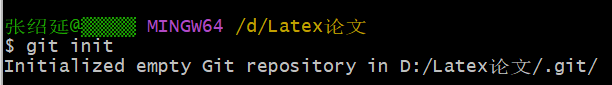
\includegraphics[width=0.5\linewidth]{git1.png}
  % 图片标题
  \captionof{figure}{初始化新仓库}
  \label{fig:example}
\end{minipage}


2.添加文件:git add .


\noindent
\begin{minipage}{\linewidth}
  \centering
  % 插入图片
  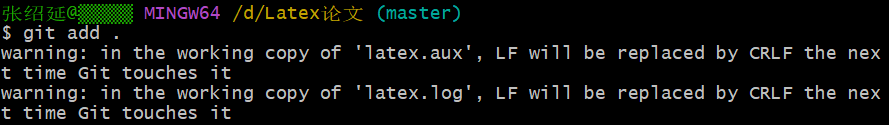
\includegraphics[width=0.5\linewidth]{git2.png}
  % 图片标题
  \captionof{figure}{初始化新仓库}
  \label{fig:example}
\end{minipage}

3.将你的 LaTeX 源文件添加到 Git 仓库:git commit -m "Initial commit of LaTeX project"

\noindent
\begin{minipage}{\linewidth}
  \centering
  % 插入图片
  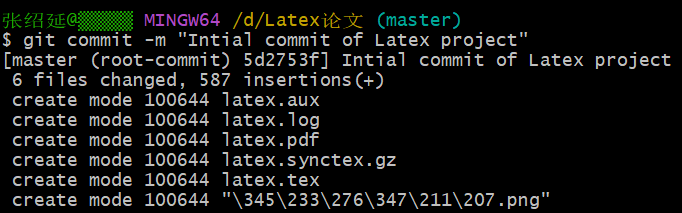
\includegraphics[width=0.5\linewidth]{git3.png}
  % 图片标题
  \captionof{figure}{初始化新仓库}
  \label{fig:example}
\end{minipage}

4.在处理大型文档或尝试新功能时,可以创建分支来隔离开发工作。

\noindent
\begin{minipage}{\linewidth}
 \centering
  % 插入图片
  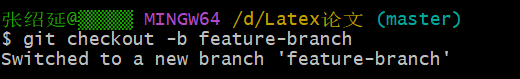
\includegraphics[width=0.5\linewidth]{git4.png}
  % 图片标题
  \captionof{figure}{初始化新仓库}
  \label{fig:example}
\end{minipage}

5.

6.

7.

8.

9.

10.


\begin{itemize}
    \item 首先,我深刻体会到……(描述你的第一个感悟)。
    \item 其次,在这次活动中,我学到了……(描述你的第二个感悟)。
    \item 最后,通过这次经历,我认识到……(描述你的第三个感悟)。
\end{itemize}

\section{解题感悟}
通过学习LaTeX,我学会了如何制作出格式规范、排版美观的文档。在撰写实验报告时,
我可以更将专注于内容创作,而不是文档的格式调整。并且LaTeX在处理数学公式和科学
符号方面非常强大,这对于学术写作和科学交流来说非常有用。通过Latex,我能够用代
码,更加容易地对文档进行维护和修改。

Git教会了我如何管理代码的历史版本,能够大大提高工作效率。首先,我学会了如何与
分支管理以及代码备份与恢复。Git提供了一个分布式的代码备份系统,这意味着即使本地文件丢失,我也可以从远程仓库恢复我的工作。
流程化和规范化:Git的使用促进了我对软件开发流程的理解,包括如何进行功能开发、问题修复和版本发布。
解决问题的能力:在遇到合并冲突或其他问题时,Git迫使我学习如何分析问题并找到解决方案,这对我的问题解决能力是一个很好的锻炼。

\end{document}
